\documentclass[12pt]{article}
\usepackage{graphicx}
\usepackage{placeins}
\usepackage{amsmath}


% acronyms for text or math mode
\newcommand {\ccast} {\mbox{\small CCAST}}
\newcommand {\cris} {\mbox{\small CrIS}}

\newcommand {\airs} {\mbox{\small AIRS}}
\newcommand {\iasi} {\mbox{\small IASI}}
\newcommand {\idps} {\mbox{\small IDPS}}
\newcommand {\nasa} {\mbox{\small NASA}}
\newcommand {\noaa} {\mbox{\small NOAA}}
\newcommand {\nstar} {\mbox{\small STAR}}
\newcommand {\umbc} {\mbox{\small UMBC}}
\newcommand {\uw}   {\mbox{\small UW}}

\newcommand {\fft}  {\mbox{\small FFT}}
\newcommand {\ifft} {\mbox{\small IFFT}}
\newcommand {\fir}  {\mbox{\small FIR}}
\newcommand {\fov}  {\mbox{\small FOV}}
\newcommand {\for}  {\mbox{\small FOR}}
\newcommand {\ict}  {\mbox{\small ICT}}
\newcommand {\ils}  {\mbox{\small ILS}}
\newcommand {\igm}  {\mbox{\small IGM}}
\newcommand {\opd}  {\mbox{\small OPD}}
\newcommand {\rms}  {\mbox{\small RMS}}
\newcommand {\zpd}  {\mbox{\small ZPD}}
\newcommand {\ppm}  {\mbox{\small PPM}}
\newcommand {\srf}  {\mbox{\small SRF}}
\newcommand {\sdr}  {\mbox{\small SDR}}

\newcommand {\ES} {\mbox{\small ES}}
\newcommand {\SP} {\mbox{\small SP}}
\newcommand {\IT} {\mbox{\small IT}}
\newcommand {\SA} {\mbox{\small SA}}

\newcommand {\ET} {\mbox{\small ET}}
\newcommand {\FT} {\mbox{\small FT}}

% abbreviations, mainly for math mode
\newcommand {\real} {\mbox{real}}
\newcommand {\imag} {\mbox{imag}}
\newcommand {\atan} {\mbox{atan}}
\newcommand {\obs}  {\mbox{obs}}
\newcommand {\calc} {\mbox{calc}}
\newcommand {\sinc} {\mbox{sinc}}
\newcommand {\psinc} {\mbox{psinc}}
\newcommand {\std} {\mbox{std}}

% symbols, for math mode only
\newcommand {\wnum} {\mbox{cm$^{-1}$}}
\newcommand {\lmax} {L_{\mbox{\tiny max}}}
\newcommand {\vmax} {V_{\mbox{\tiny max}}}

\newcommand {\tauobs} {\tau_{\mbox{\tiny obs}}}
\newcommand {\taucal} {\tau_{\mbox{\tiny calc}}}
\newcommand {\Vdc}  {V_{\mbox{\tiny DC}}}

\newcommand {\rIT} {r_{\mbox{\tiny\textsc{ict}}}}
\newcommand {\rES} {r_{\mbox{\tiny\textsc{es}}}}
\newcommand {\robs} {r_{\mbox{\tiny obs}}}

\newcommand {\rITobs} {r_{\mbox{\tiny\textsc{ict}}}^{\mbox{\tiny obs}}}
\newcommand {\rITcal} {r_{\mbox{\tiny\textsc{ict}}}^{\mbox{\tiny cal}}}

\newcommand {\ITmean} {\langle\mbox{\small IT}\rangle}
\newcommand {\SPmean} {\langle\mbox{\small SP}\rangle}



\title{A Note on Interferometric Calibration \\
\vspace{3mm}
{****} DRAFT {****} \\
}

\author{H.~E.~Motteler and L.~L.~Strow \\
  \\
  UMBC Atmospheric Spectroscopy Lab \\
  Joint Center for Earth Systems Technology \\
}

\date{\today}
\begin{document}

\maketitle

We consider the definition of reference truth for measurements made
with a Michelson interferometer, taking into account relatively
small (or possibly non-existant) effects such as filter position and
potential mathematical artifacts.  The immediate application is
defining reference truth and a corresponding calibration equation
for the for the {\cris} instrument.

% We want to be careful with definitions to separate mathematical
% and physical artifacts in subsequent derivations.

% pedantic because looking for small effects

\section{Michelson Interferometer}

\begin{figure}
  \centering
  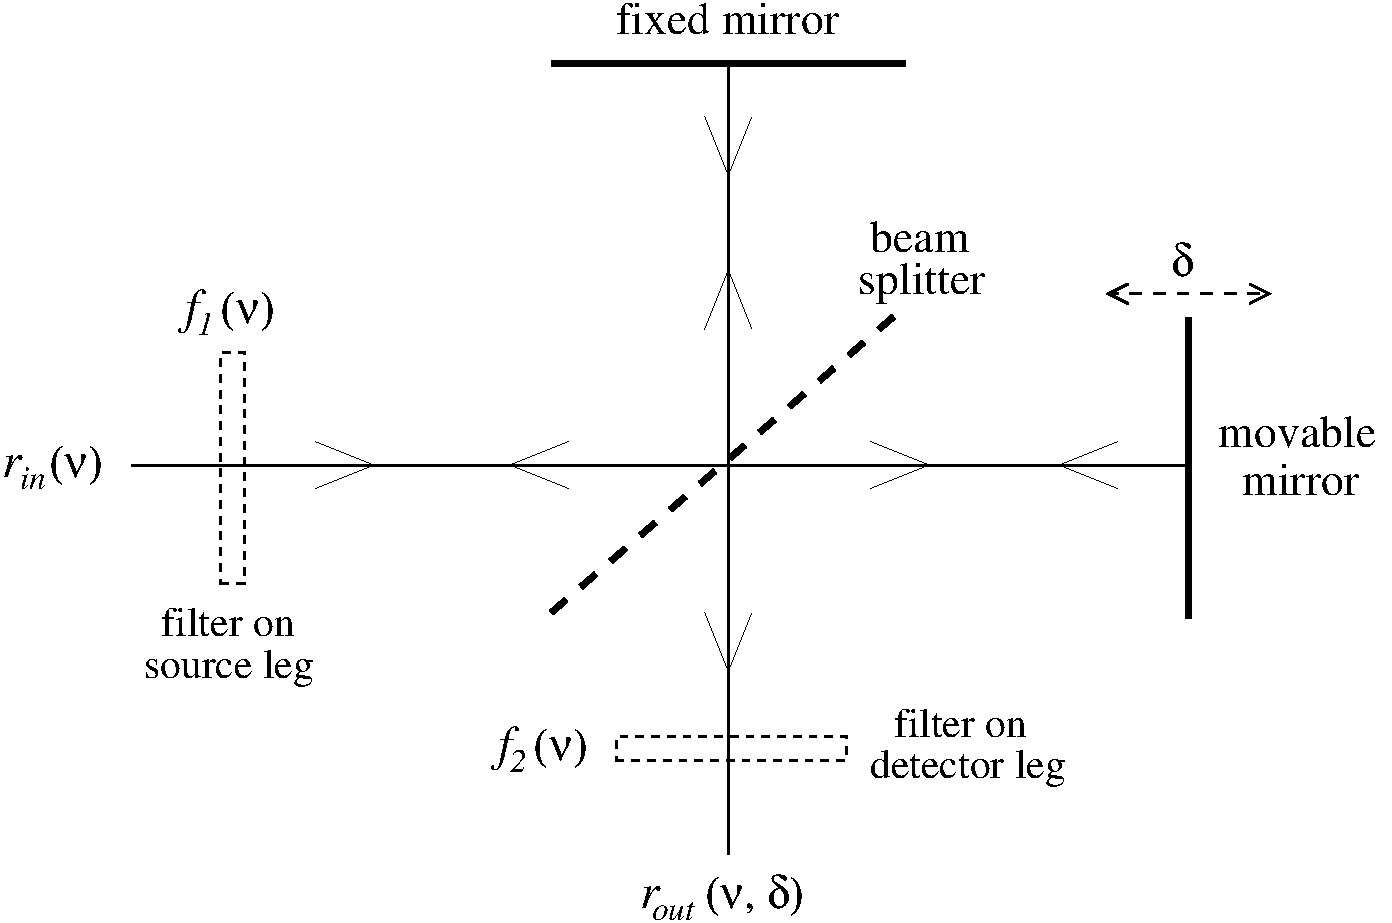
\includegraphics[scale=0.5]{figures/mich_filt2.pdf}
  \caption{Michelson interferometer with filters}
  \label{intf1}
\end{figure}

Figure \ref{intf1} shows a basic Michelson interferometer.  Let
$\rin(\nu)$ be incoming radiance as a function of frequency $\nu$,
$\delta$ mirror displacement, and $\rout(\nu, \delta)$ radiance on
the path to the detector.  In practice the signal from the detector
is the product of incoming radiance, beam-splitter efficiency, and
detector responsivity.  But suppose for the moment that we have a
perfect beam splitter and mirrors, and that there are no filters.
Then radiance $\rout$ on the path to the detector can be represented
as

\begin{equation}\label{eq1}
  \rout(\nu,\delta) = \rin(\nu)(1+\cos 2\pi\nu\delta)/2
\end{equation}

\noindent
including a term $\rin(\nu)/2$ that depends only on $\nu$.
Integrating over frequency, we have

\begin{equation}\label{eq2}
  \rout(\delta) = \frac{1}{2}\int_{\nu=0}^{\inf}\!\rin(\nu)d\nu + 
     \frac{1}{2}\int_{\nu=0}^{\inf}\!\rin(\nu)\cos(2\pi\nu\delta)d\nu
\end{equation}
\noindent
This is the continuous interferogram as a function of
displacement~$\delta$.  

We are interested in the following question: if we have a single
filter $f(\nu)$, does $\rout$ (output radiance, in our diagram)
change when $f$ is moved from the input to the detector leg of the
interferometer?  We present two related arguments that it does not.
Consider figure \ref{intf1} again, and suppose we have $f =
f_1(\nu)$ on the input leg and nothing on the output leg.  This can
be represented as

\begin{equation}\label{eq3}
  \rout(\nu,\delta) = f(\nu)\rin(\nu)(1+\cos 2\pi\nu\delta)/2
\end{equation}

Now suppose we move $f$ to the detector leg.  The assumption in the
literature seems to be that equation (\ref{eq3}) stll holds.  Note
that filter position does not matter for the $\rin(\nu)/2$ term, or
for the case when we remove one of the mirrors.

Consider two lines at frequencies $\nu_1$ and $\nu_2$, where $\nu_1$
is in the passband of $f$ and $\nu_2$ is not.  If $f$ is on the
detector leg then both $\nu_1$ and $\nu_2$ will participate in
interference, with radiance before the filter as in equation
(\ref{eq1}).  After the filter we have $\rout(\nu_2,\delta) = 0$ for
all $\delta$, with $\rout(\nu_1,\delta)$ unchanged.  If $f$ is on
the input leg then $\nu_1$ will be as before but $\nu_2$ will not be
present anywhere downstream, so again we have $\rout(\nu_2,\delta) =
0$ for all $\delta$.  So the cases are the same.

Note that in this hypothetical situation there is no nonlinearity or
intermodulation because we are assuming a perfect beamsplitter and
mirrors, and no Nyquest limit, truncation, or discretization errors
because we are considering the case for arbitraly real-valued
$\delta$.  But the argument may not apply as $\nu_1 \rightarrow
\nu_2$, because at some point $f$ can not separate them.

The case we are interested in practice is where $\nu_1$ and $\nu_2$
are close and fall on a slope or shoulder of $f$.  But for the
following argument we don't need to assume that.  So consider the
case of arbitrary $\nu_1$ and $\nu_2$.  The AC component of equation
(\ref{eq2}) with $f$ on the input leg is

\begin{equation}\label{eq4}
  \rout(\delta) = \int_{\nu=0}^{\inf}f(\nu)\cos(2\pi\nu\delta)d\nu
\end{equation}

\noindent
For the case where $\nu$ takes on only the two values $\nu_1$ and
$\nu_2$ this simplifies to

\begin{equation}\label{eq5}
  \rout(\delta) = f(\nu_1)\cos(2\pi\nu_1\delta) + 
                  f(\nu_2)\cos(2\pi\nu_2\delta)
\end{equation}

\noindent
This is interesting because of the recognizable beat pattern in 
the interferogram.  Now consider $f$ on the output leg.  On the 
path before $f$ we have the case of no filter,

\begin{equation}\label{eq6}
  \rout(\delta) = \cos(2\pi\nu_1\delta) + 
                  \cos(2\pi\nu_2\delta)
\end{equation}

\noindent
And after $f$ we have equation (\ref{eq5}) again.  Since $\nu_1$ and
$\nu_2$ were chosen arbitrarily we conclude that the property holds
for all $\nu$ and $\delta$, and that the filter position does not
matter.

In practice, $f_1$ might be beam splitter efficiency, $f_2$ detector
responsivity, and $g(\rout(\delta))$ a function taking radiance to
voltage.  In the case of the {\cris} instrument, $f_2$ could be
detector responsivity plus optical filter effects.  The particular
question for {\cris} we were interested in was if it was correct
to model the effects of a filter on the detector leg with a filter
on the input.  The answer seems to be yes.

\FloatBarrier

\section{CrIS reference truth }

\begin{figure}
  \centering
  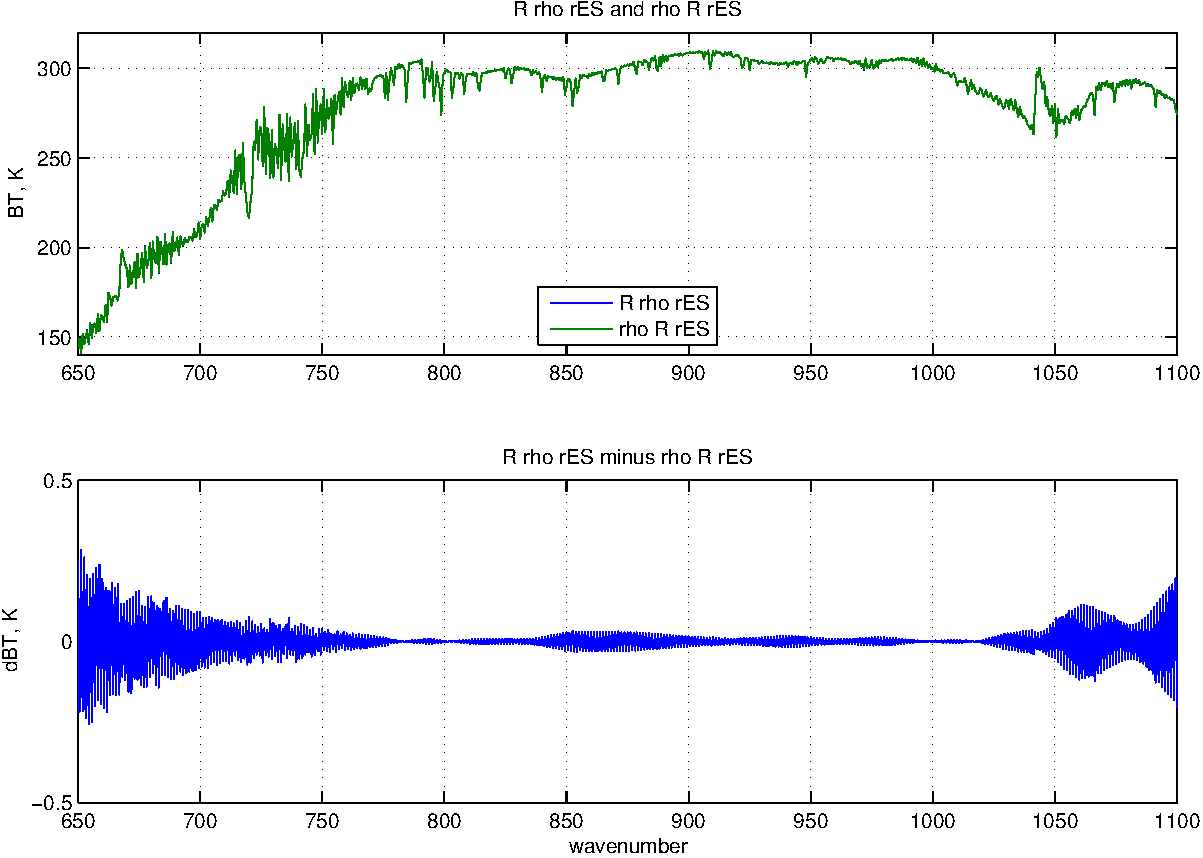
\includegraphics[height=8cm]{figures/ES_comm.pdf}
  \caption{$R\rho\,\rES$ and $\rho\,R\,\rES$}
  \label{ESdif}
\end{figure}

\begin{figure}
  \centering
  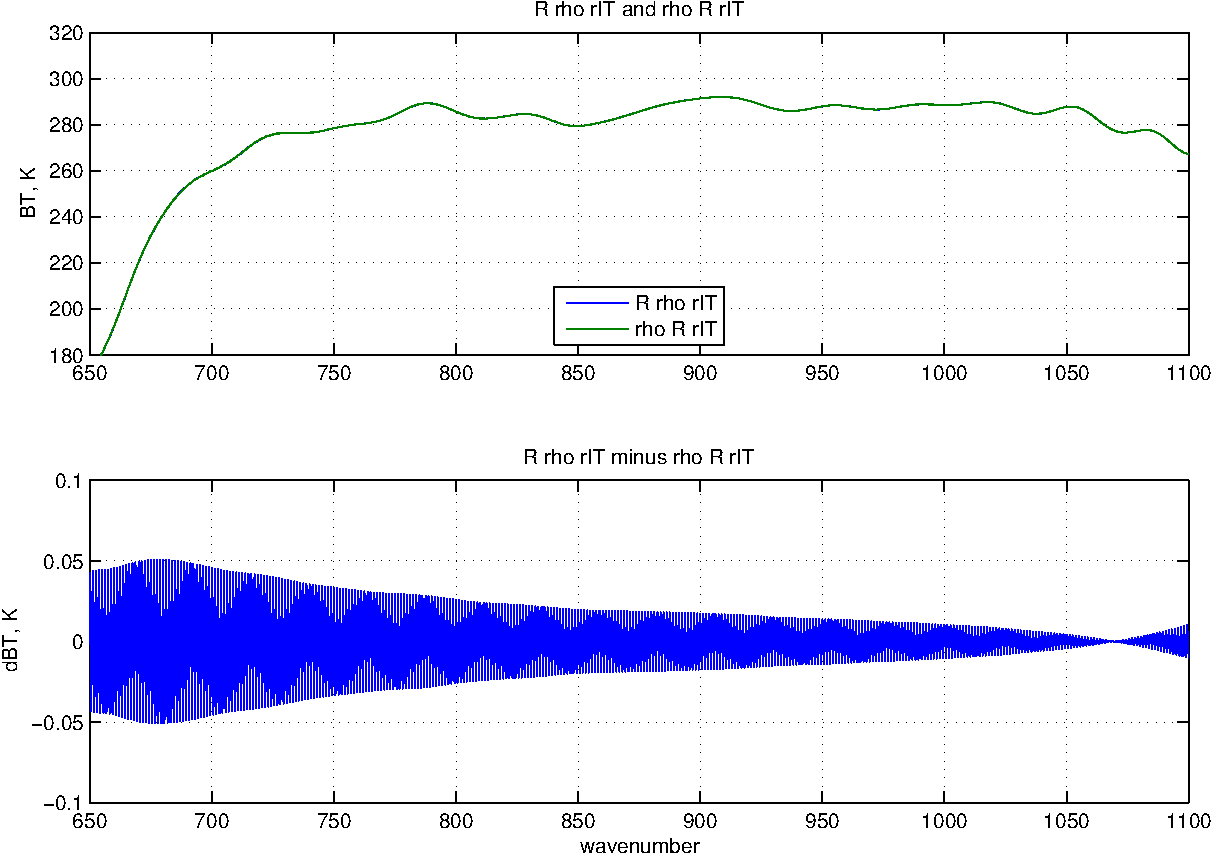
\includegraphics[height=8cm]{figures/BB_comm.pdf}
  \caption{$R\rho\,\rIT$ and $\rho\,R\,\rIT$}
  \label{BBdif}
\end{figure}

We can a derive reference truth from a basic form of the {\cris}
calibration equation, with details depending on assumptions about
instrument behavior.  Suppose $\rES$ is high resolution earth scene
radiance, $\rIT$ high resolution black-body radiance from the
internal calibration target, $\rho$ instrument responsivity, and $R$
resampling from high resolution to the instrument sensor grid.

% $dv = 1/ (2\, \opd)$, where $\opd$ is the maximum optical path
% difference.

If $r$ is some arbitrary high resolution radiance, we might expect
that $R\rho\,r \approx \rho R\,r$.  Figure \ref{ESdif} shows the
difference for a typical earth scene, and figure \ref{BBdif} the
difference for an {\ict} (black body) look.  Suppose we interpret
this as $R\rho\,\rIT \approx \rho\,R\,\rIT$ for ICT looks, but
$R\rho\,\rES \ne \rho\,R\,\rES$ for earth scenes.  Calibration of
the on-axis optical path of a Michaelson interferometer can be
represented as

\begin{equation}\label{caldef}
  \rcalLR = \rITLR  \frac{\ES - \SP}{\IT - \SP}
\end{equation} 

\noindent
where $\rcalLR$ is calibrated radiances, $\rITLR$ is expected
radiance from the internal calibration target, and $\ES$, $\IT$, and
$\SP$ are uncalibrated spectra for earth scene, internal calibration
target, and space looks, respectively.  Note that all values in
equation \ref{caldef} are at the ``sensor grid'' $dv = 1/ (2\,
\opd)$.

Let $\ES \approx R\rho(\rES+\rSP)$, $\IT \approx R\rho(\rIT+\rSP)$,
and $\SP \approx R\rho\,\rSP$, where $\rES$, $\rIT$, and $\rSP$ are
high resolution approximations to the true radiances, $\rho$ is
responsivity, and $R$ is resampling from the high resolution to the
sensor grid $dv$.  Let $\rITLR = R(\rIT)$.  Substituting this into
(\ref{caldef}) gives

\begin{align}
  \rcalLR &\approx \rITLR \frac{R\rho(\rES+\rSP) - R\rho\,\rSP}
                               {R\rho(\rIT+\rSP) - R\rho\,\rSP} \notag \\
%         &= \rITLR \frac{R\rho\,\rES + R\rho\,\rSP - R\rho\,\rSP}
%                        {R\rho\,\rIT + R\rho\,\rSP - R\rho\,\rSP} \\
          &= \rITLR \frac{R\rho\,\rES}
                         {R\rho\,\rIT} \label{cal1} \\
          &\approx \rITLR \frac{R\rho\,\rES}
                               {\rho\,R\,\rIT} \label{cal2} \\
          &= \frac{R\rho\,\rES} 
                  {\rho} = \rresp \label{calUW}
\end{align} 

\noindent
We go from equation \ref{cal1} to \ref{cal2} because we have assumed
responsivity commutes at least approximately with resampling for the
ICT look.   Equation \ref{calUW} is the UW definition of ``reference
truth with responsivity''.

\vspace{2mm}
A more conventional and user-friendly definition of reference truth
is
\begin{equation}
  \rflat =  R \: \rES
\end{equation} 

\noindent
If we assume $R\rho\,\rES \approx \rho\,R\,\rES$ then we get
``flat'' reference truth.  In practice we find the ``ratio first''
\umbc\ \ccast\ reference calibration equation has smaller residuals
when compared with $\rflat$, while the ``$\SA^{-1}$ first'' \noaa~4
algorithm has smaller residuals with $\rresp$.  It seems to us the
proper focus for calibration algorithm development should be
minimizing residuals in comparison with~$\rflat$.

\newpage
\section{Resampling}

We often use double Fourier interpolation to move from one frequency
grid to another [4].  For interpolation from a relatively fine grid
(for example a step of $0.0025$ \wn) to a typical instrument grid
this gives an $O(n \log n)$ algorithm.  But for two relatively close
grids we may get better runtimes with a resampling matrix.  Perhaps
the simplest way to represent such a matrix is with an explicit sinc
basis,

\begin{equation}\label{res1}
  R(i,j) = \frac{dv_s}{dv_u}\cdot
      \sinc(\displaystyle \frac{v_s(j) - v_u(i)}{dv_u})
\end{equation} 

\noindent
Here $v_s$ is an $n$--vector of sensor-grid frequencies, $v_u$ an
$m$--vector of user-grid frequencies, $dv_s$ the sensor-grid
spacing, and $dv_u$ the user-grid spacing.  $R$~is an $m \times n$
matrix whose columns correspond to sensor-grid channels and rows to
user-grid channels.  $R$ is applied as $r_u = R \: r_s$, where $r_s$
is an $n$--vector of sensor-grid radiances and $r_u$ an $m$--vector
of user-grid radiances.  One way to see this works is to note that
an impulse at a sensor grid channel gives a sinc function sampled at
the user grid, and that a linear transform is uniquely determined by
its action on an orthogonal basis.  

$R$ defined this was is a close cousin to the {\cris} SA matrix.
The key difference is that for the SA matrix we have an ILS rather
than pure sinc basis.  The limit as $dv_u \rightarrow dv_s$ gives
the identity matrix.  In that case we still have a sinc basis, but
values for $i\ne j$ are sampled at the zero crossings.
In practice equation (\ref{res1}) gives good agreement with double
Fourier interpolation.  For the NOAA 18-20 Jan 2016 test the mean
difference was less than $0.01$K in the SW and less than $0.002$K
for the MW and LW {\cris} bands.

% since each column of $R$ is associated with a sinc function whose
% center is at a sensor-grid frequency, evaluated at the user-grid
% frequencies.

The NOAA/MIT {\cris} resampling function is

\begin{equation}\label{res2}
  R(i,j) = \frac{dv_s}{dv_u}\cdot
     \frac{\sin(\displaystyle \pi \frac{v_s(j) - v_u(i)}{dv_u})}
  {N \cdot \sin(\displaystyle \pi \frac{v_s(j) - v_u(i)}{N \cdot dv_u})}
\end{equation} 

\noindent
For {\cris} the convention seems to be to take $N = n \times d$ for
a band-dependent decimation factor $d$ of roughly 20.  This also
gives a good approximation to double Fourier interpolation.  Note
that $N\cdot \sin(c/N) \approx N \cdot c/N$ for large $N$, so the
limit as $N\rightarrow\inf$ of $N\cdot \sin(c/N)$ is $c$.  Applying
this to equation (\ref{res2}) we see the limit as $N\rightarrow\inf$
gives equation \ref{res1}, and in practice the resulting matrices
are very close for {\cris} with $N = n \times d$.

% columns correspond to sensor grid channels and the rows to user grid
% channels.  Each column is associated with a sinc function whose
% center is at the sensor grid channel frequency, while each row is
% those sinc functions evaluated at the user grid channel frequencies.

\end{document}

